\documentclass{iscs}
\begin{document}
\title{When Observation Choices Resemble Dynamics\\in AI Conversation Archives}
\titlerunning{Observation Choices in AI Conversations}
\authors{\speaker{Alexander Richard Towell}}
\authorsrunning{A. R. Towell}
\addresses{Southern Illinois University Edwardsville, Edwardsville, IL, USA; lex@metafunctor.com}
\abstract{We revisit conversation-network and embedding measurements through their observation process. Fixed-graph revelation has mechanical growth expectations, while matched forecast origins change a user--assistant history contrast on exposed PRISM data. These case studies support explicit reporting of observation units, available information and controls before interpreting structure as cognitive dynamics.}
\keywords{Conversation networks; Semantic embeddings; Temporal nulls; Measurement; Human--AI interaction}
\maketitle\unskip\par

\section{From archive maps to claims about development}
Conversation archives support useful representations of human--AI interaction,
but a representation's evolution need not identify the process that generated
the interaction. The published Cognitive MRI case study constructed a semantic
similarity network and described communities and bridge conversations
\cite{towell2026cmri}. The accepted ISCS 2026 hierarchy study related episodes
to extracted concepts and interpretably chosen abstraction levels
\cite{towell2026hierarchy}. Both draw on the same 1,908-conversation author
archive; they are not independent replications. Their descriptive constructions
motivate, but do not validate, measurements of memory, learning or intellectual
influence.

We synthesize two completed calibration studies around one question:
\emph{which apparent dynamics depend on how an archive becomes observable?}
The first concerns revealing vertices of a fixed endpoint graph; the second
concerns which messages are available when forecasting the next contribution.
The contribution is an auditable methodological case study linking network and
sequence measurements, with explicit limits on cognitive interpretation.
No new conversations or confirmation sample are introduced here.

\section{Revelation of a fixed graph already produces growth}
Let $G$ be a fixed simple graph on $N\geq2$ conversation vertices with $M$ edges
and degrees $d_i$. Whole-conversation embeddings and a fixed similarity threshold
determine its edges. Reveal vertices in a uniformly random order and retain
the induced graph after $k$ arrivals. Its edge count $M_k$ satisfies
\begin{equation}
\mathbb{E}[M_k]=M\frac{k(k-1)}{N(N-1)}.
\label{eq:edges}
\end{equation}
Each endpoint pair is included with the same probability, so linearity of
expectation gives this result for every endpoint graph. Clustering is not
required. A growing edge curve alone therefore cannot distinguish semantic
development from graph revelation.

The vertex denominator also matters. All arrivals number $k$, whereas active
vertices $A_k$ exclude isolates. For $1\leq k\leq N$,
\begin{equation}
\mathbb{E}[A_k]=\sum_{i=1}^{N}\frac{k}{N}
\left[1-\frac{\binom{N-1-d_i}{k-1}}{\binom{N-1}{k-1}}\right].
\label{eq:active}
\end{equation}
The term in brackets is the probability that an included vertex has an included
neighbor. We verified both identities by exhaustive subset enumeration of
small graphs, including isolates and complete graphs, using the existing
calibration implementation. These are expectation identities, not formulas
for the expected slope of a fitted log--log regression.

Population-versus-activity distinctions already occur in temporal-network
densification research \cite{kobayashi2020}; structured temporal reference
models are established \cite{gauvin2022}. Their application here requires
declaring which order information is destroyed. Uniform permutations and
block reorderings that retain internal order answer different questions. A residual
under either control remains conditional on its exchangeability assumptions;
nonrejection does not establish that all observed growth is mechanical.
Likewise, placing a completed conversation's features at its creation time is
retrospective observation unless feature availability is independently established.

\section{Forecast origin changes a role contrast}
The second case reuses exposed development results from PRISM
\cite{kirk2024}: 1,191 selected conversations in 360 dependence components,
grouped using participant identifiers and duplicate links. These are grouping
proxies, not independently verified longitudinal individuals. The probe portion
contains 240 conversations in 72 components and 428 paired user/assistant
targets. Earlier fit and tuning partitions contain 216 and 72 components.
All these data were inspected in previous pilots; the separate 248-component
reserve remains unused.

For each target, we compare normalized uniform pooling of available message
vectors with pooling the last two messages. Let $g_r$ be the mean difference
in target cosine similarity for role $r$, and let $I=g_{\mathrm{assistant}}-
g_{\mathrm{user}}$. Message positions and target embeddings are fixed. The
native view uses at most the first 128 content tokens per message, with targets
after at least two completed exchanges and within the first twelve messages.
MiniLM-L6-v2 and E5-small-v2 are two instruments on the same data.

The \emph{natural} origin includes every message before each target: assistant
prediction sees the current user request. The \emph{common-prefix} origin
predicts both members of a pair from the same preceding completed exchange,
withholding that request. User predictions are unchanged. Assistant prediction
now has a longer forecast horizon, so this comparison does not isolate a causal
effect of human versus artificial memory.

\begin{figure}[ht]
\centering
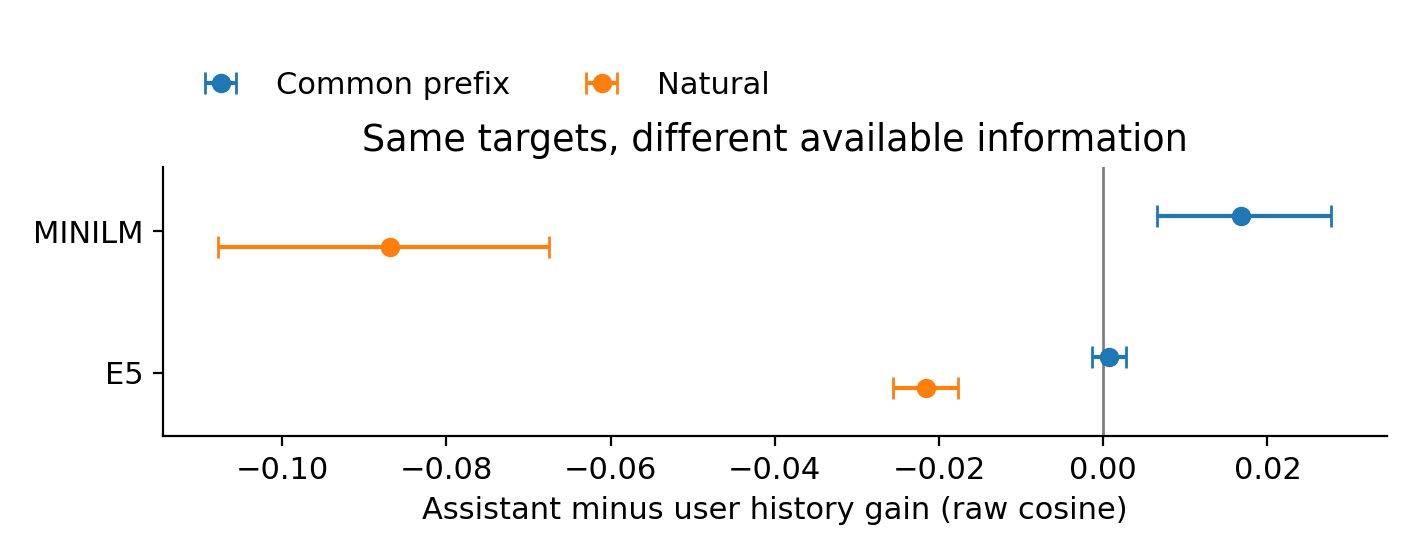
\includegraphics[width=\linewidth]{figures/forecast-origin.png}
\caption{Role interaction $I$ in the native input view. Bars are descriptive
95\% component-bootstrap intervals (2,000 draws), conditional on the exposed
development sample. Positive values mean a larger mean-versus-last-two gain
for assistant targets. Encoder scales need not be comparable. Changing origin
withholds information and changes the assistant forecast horizon.}
\label{fig:origin}
\end{figure}

Under natural origins, $I=-0.0869$ for MiniLM and $-0.0215$ for E5.
Under the common prefix, the values become $+0.0168$ and $+0.0006$
(Fig.~\ref{fig:origin}). The ordering reverses for MiniLM; E5 is near zero
with an interval spanning zero. We do not claim every role difference vanishes.
Meanwhile, next-user mean-history gains remain positive: $0.0344$
[$0.0225,0.0488$] for MiniLM and $0.0192$ [$0.0160,0.0226$] for E5.
The earlier fixed checks also retain positive user gains with expanded text,
restored message weighting after chunking, and exposure to valid past response
candidates. The case constrains a role interpretation while preserving a
useful predictive measurement.

Uncertainty averages targets within conversations and conversations within
components, then resamples components with equal weight. It does not treat
428 target pairs as independent people. Synthetic controls from the completed
study reproduce a history benefit with a fixed topic and conditionally
independent user innovations; a process with planted older-state dependence
also produces it. Thus the cosine contrast does not identify a memory mechanism.
It is not an accuracy measure for reasoning, learning or useful assistance.

\section{Contribution boundary and reporting implications}
Curved Contrastive Learning already reports dialogue-intent-dependent benefits
of full versus recent history \cite{erker2023}. OnePred compares history and
intent-memory approaches to next-query prediction \cite{chen2026onepred}.
Our synthesis does not claim priority for useful context, role differences or
temporal nulls. Its practical contribution is to show, with exact graph
identities and a quantified forecast-origin contrast, why the observation
process must accompany an interpretation of conversational dynamics.

A report should specify the unit retained, when its features become available,
the population denominator, the permitted predictive prefix, and what each
control preserves. Graph revelation and forecast withholding are distinct
operations; their common lesson is that a changed measurement can reflect a
changed observable rather than a changed underlying mechanism. This supports
more accountable use of conversation-derived profiles in research and AI memory
design, without claiming a demonstrated downstream benefit.

This synthesis combines published descriptive work, established mathematics
and exposed development analyses. It establishes neither natural prevalence
nor a general theory of memory or semantic dynamics. The evidence package
records source versions, all four forecasting views, component effects and
replay checks. A stronger empirical paper needs a distinct outcome and
independent evidence. This synthesis does not justify reserve evaluation.

\bibliography{references}
\end{document}
